\section{Current Status}
\sectionframe

\subsection{Materials}
\begin{frame}{Magnetism in van der Waals materials}
	\begin{columns}
		\column{.7\textwidth}
		\centering
		\includegraphics[width=\textwidth]{image11.png}\\
		\small\raggedleft Magnetism in two-dimensional van der Waals materials, Nature 2018

		\column{.3\textwidth}
		"While \emph{MnPS3} is best described by the \emph{isotropic Heisenberg Hamiltonian}, \\
		\emph{FePS3} is most effectively treated by the \emph{Ising model}, \\
		while \emph{NiPS3} is best described by the \emph{anisotropic Heisenberg Hamiltonian}."\\
		\vspace{1cm}
		\small\raggedleft
		Magnetism in the layered transition-metal thiophosphates MPS3 (M =Mn, Fe, and Ni), Physical Review B 1992
	\end{columns}
\end{frame}

\begin{frame}{NiPS$_3$}
	\centering
	\includegraphics[width=.8\textwidth]{image13.png}
	\\\vspace{1cm}
	\small\raggedleft
	Exciton-driven antiferromagnetic metal in a correlated van der Waals insulator,
	Nature Communications 2021
\end{frame}

\subsection{Setup}
\begin{frame}{Setup}
	\centering
	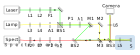
\includegraphics{../figures/setup.pdf}
\end{frame}


\subsection{Photoluminescence and Reflection at 0 T}
\begin{frame}{bulk PL spectra at 10 K}
	\centering
	\includegraphics{../figures/2023-12-10 Combined PL.pdf}
\end{frame}

\begin{frame}{Reflectance spectra}
	\centering
	\includegraphics{../figures/2023-12-10 reflectance.pdf}
\end{frame}

\begin{frame}
	\begin{columns}
		\column{.3\textwidth}
		\centering
		\includegraphics[width=\textwidth]{../figures/sample_photos/i001_MnPS3_50x_a.png}
		MnPS$_3$ Bulk Crystal (50x)

		\column{.3\textwidth}
		\centering
		\includegraphics[width=\textwidth]{../figures/sample_photos/i005_NiPS3_50x.png}
		NiPS$_3$ Bulk Crystal (50x)

		\column{.3\textwidth}
		\centering
		\includegraphics[width=\textwidth]{../figures/sample_photos/exfoliated_NiPS3.png}
		NiPS$_3$ Exfoliated Crystal
	\end{columns}

\end{frame}


\subsection{NiPS$_3$ in magnetic field}
\subsubsection{in plane}
\subsectionframe

\begin{frame}{Instability of the Lens assembly?}
	\begin{columns}
		\column{.6\textwidth}
		\centering
		\includegraphics{../figures/2023-12-10 lens movement.pdf}

		\column{.3\textwidth}
		\begin{figure}
			\centering
			\includegraphics[width=\textwidth]{../figures/sampleHolder.pdf}
			Field in plane of the image.
		\end{figure}
	\end{columns}
\end{frame}

\begin{frame}{Splitting of the PL peak at $\measuredangle P,H=0$}
	\begin{columns}
	\column{.5\textwidth}
	\centering
	\includegraphics{../figures/2023-12-10 splitting.pdf}
	\column{.5\textwidth}
	\centering
	\includegraphics{../figures/2023-12-10 splitting quantified.pdf}
	\end{columns}
\end{frame}


\begin{frame}{Polarisation}
	\centering
	% \includegraphics{../figures/2023-12-10 splitting polarisation on 2023-12-06_LO_MG_NiPS3 d004_10K_647nm_rotPolDet_flake05_sweepDown_inPlane.hd5.pdf}
	\includegraphics{../figures/2023-12-10 splitting polarisation on 2023-12-06_LO_MG_NiPS3 d004_10K_647nm_rotPolDet_flake05_sweepDown_inPlane.hd5.pdf}
\end{frame}
\begin{frame}{at 50K}
	\centering
	\includegraphics{../figures/2023-12-10 splitting polarisation on 2023-12-08_LO_MG_NiPS3 d001_flake04_50K_inPlane_linPol_sweepUp.pdf}
\end{frame}

\begin{frame}{Understanding in Plane field}
	\begin{columns}
		\column{.3\textwidth}
		My measurement:\\\vspace{1cm}
		\centering
		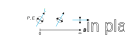
\includegraphics{../figures/vector_rotation.pdf}
		\\\vspace{1cm}\raggedleft\small
		Based on Fig. 4 b in Spin-induced linear polarization of photoluminescence in antiferromagnetic van der Waals crystals, Nature Materials 2021
		\column{.7\textwidth}
		\centering
		\includegraphics[width=\textwidth]{image12.png}

	\end{columns}
\end{frame}

\subsubsection{out of plane}
\begin{frame}{Out of plane field}
	\centering
	\includegraphics{../figures/2023-12-10 circular dichroism 2023-12-11_NiPS3 d002_flake04_50K_circPol_inPlane.pdf}
\end{frame}

\subsection{CrPS$_4$}
\subsectionframe

\begin{frame}{excitation power dependence}
	\centering
	\includegraphics{../figures/2023-12-14 CrPS4 excitation power dependence.png}
\end{frame}

\begin{frame}{CrPS$_4$: $CD \propto M$ ?}
	\begin{columns}
		\column{.5\textwidth}
		My measurement:\\
		\centering
		\includegraphics{../figures/2023-12-14 CrPS4 circular dichroism.pdf}
	
		\column{.5\textwidth}
		\centering
		\includegraphics[width=\textwidth]{image14.png}
		\\\vspace{1cm}\raggedright\small
		Magnetic Structure and Metamagnetic Transitions in the van der Waals
		Antiferromagnet CrPS$_4$, Advanced Materials 2020

	\end{columns}
	
\end{frame}


\begin{frame}{moving flakes}
	\begin{columns}

		\column{.5\textwidth}
		\centering
		\includegraphics{../figures/2023-12-14 flake turning linear polarisation.pdf}


		\column{.5\textwidth}
		\centering
		\begin{figure}
			\includegraphics[width=\textwidth]{../../data/2023-12-14_CrPS4_outPlane/flake03_rotation_cropped.png}
			\caption{Flake 03, background: flake after cooldown, foreground: flake before, rotated by 30°}
		\end{figure}
	\end{columns}

\end{frame}

\begin{frame}{Linear Polarisation}
	\centering
	\includegraphics{../figures/2023-12-15 CrPS4 linear dichroism.pdf}
\end{frame}


\section{Writing}
\sectionframe
